% Appendix page
\newpage
\section*{Appendix A}
\addcontentsline{toc}{section}{Abstract}

\begin{figure}[h]
  \centering
    
\includegraphics[width=1\textwidth]{fig/home_screenshot.png}
    \caption{Home Page Screen-shot.}
\end{figure}

\newpage
\begin{figure}[h]
  \centering
    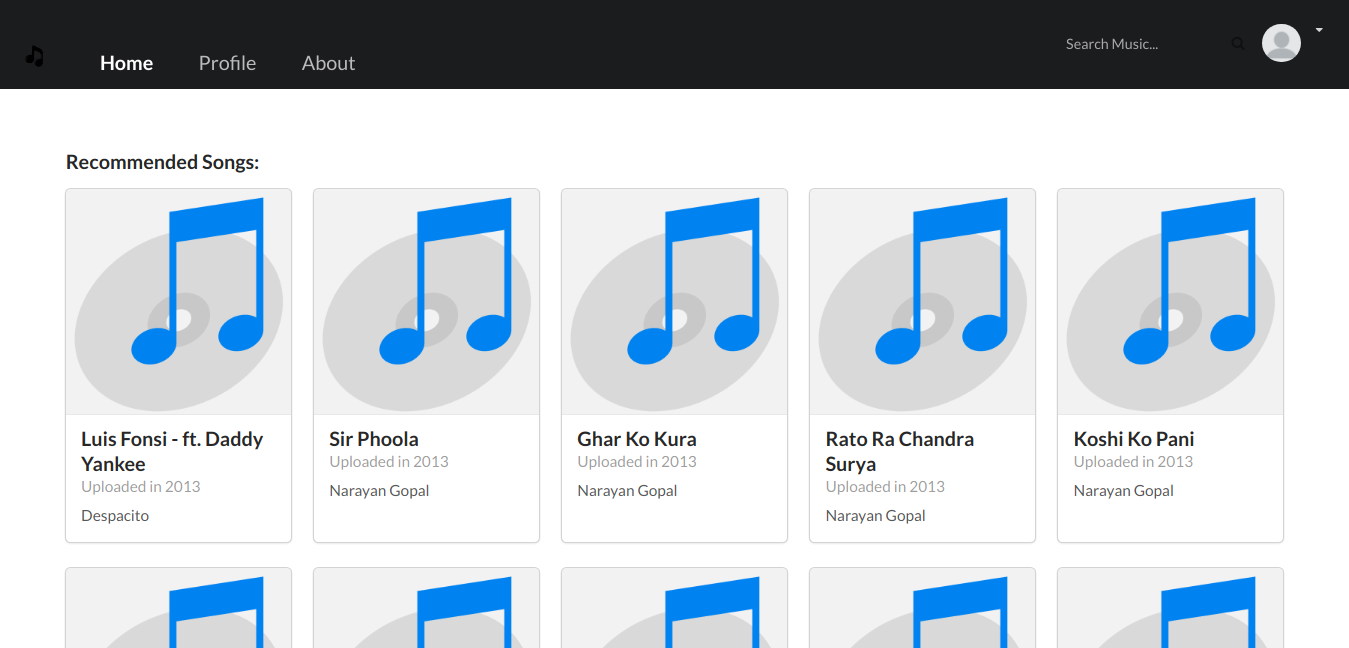
\includegraphics[width=1\textwidth]{fig/recommended_songs.png}
    \caption{Recommended Songs Page.}
\end{figure}

\newpage
\begin{figure}[h]
  \centering
    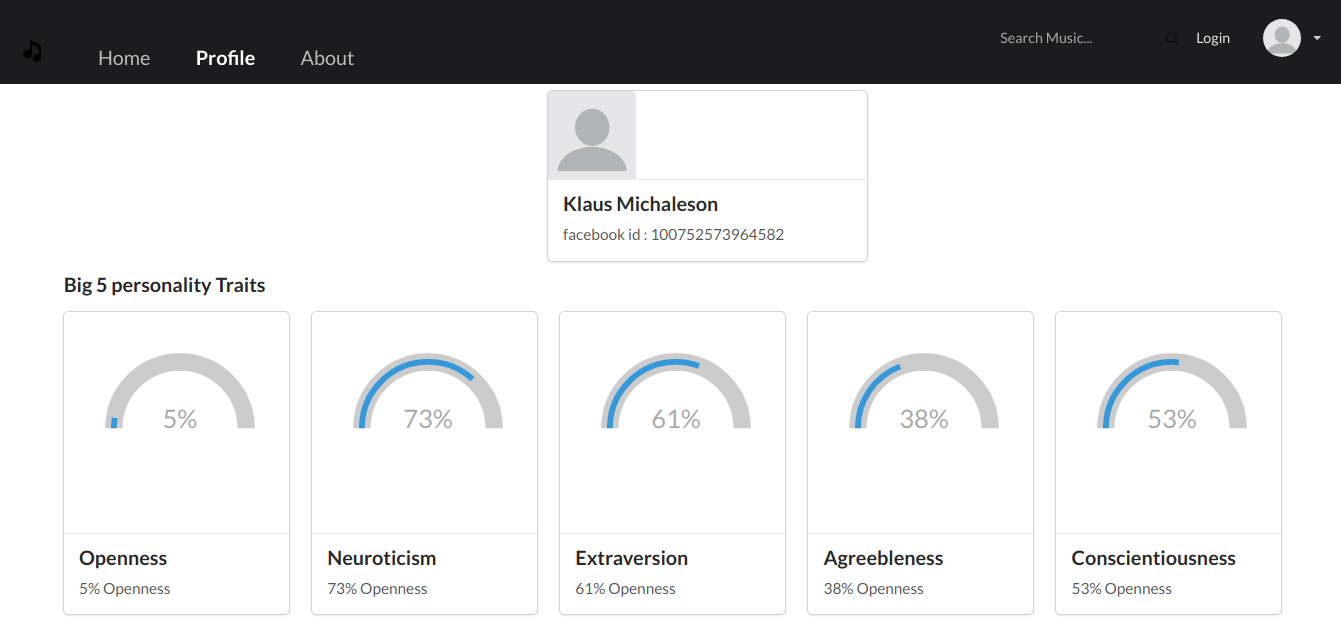
\includegraphics[width=1\textwidth]{fig/profile_screenshot.png}
    \caption{User Profile Page.}
\end{figure}

\newpage
\begin{figure}[h]
  \centering
    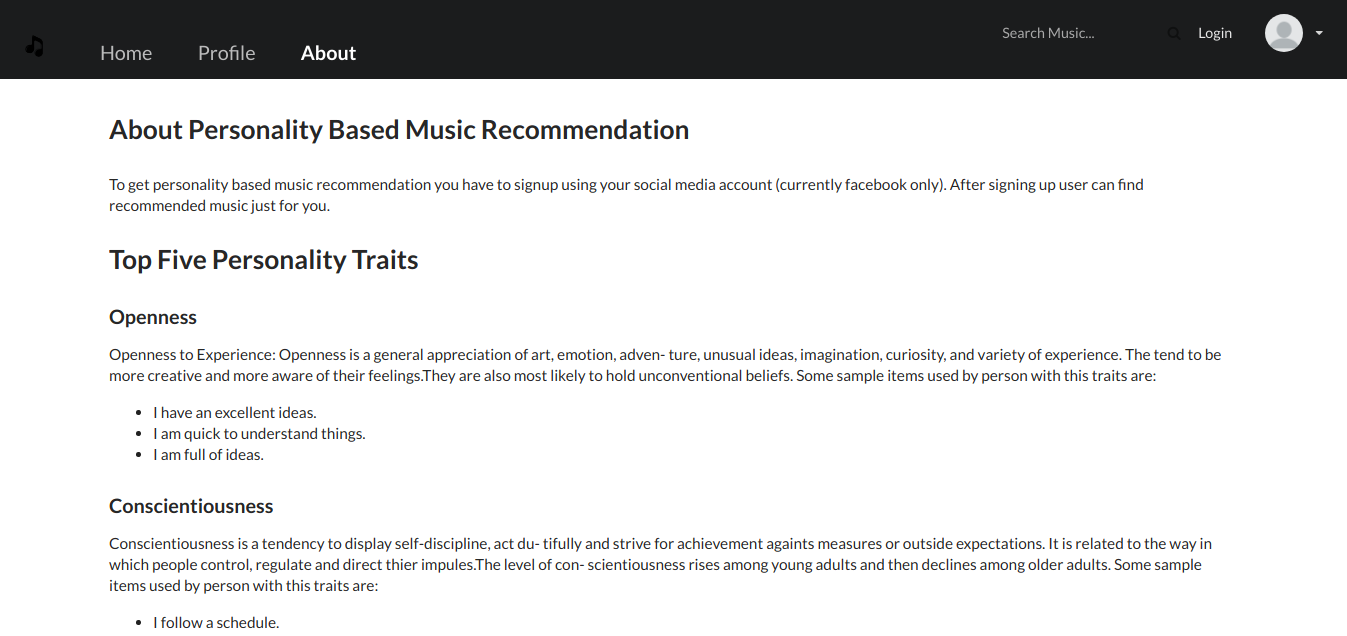
\includegraphics[width=1\textwidth]{fig/help_screenshot.png}
    \caption{Help Page.}
\end{figure}

\newpage
\section*{Appendix B}
Stopwords used\\
{\em 'i', 'me', 'my', 'myself', 'we', 'our', 'ours', 'ourselves', 'you', 'your', 'yours', 'yourself', 'yourselves', 'he', 'him', 'his', 'himself', 'she', 'her', 'hers', 'herself', 'it', 'its', 'itself', 'they', 'them', 'their', 'theirs', 'themselves', 'what', 'which', 'who', 'whom', 'this', 'that', 'these', 'those', 'am', 'is', 'are', 'was', 'were', 'be', 'been', 'being', 'have', 'has', 'had', 'having', 'do', 'does', 'did', 'doing', 'a', 'an', 'the', 'and', 'but', 'if', 'or', 'because', 'as', 'until', 'while', 'of', 'at', 'by', 'for', 'with', 'about', 'against', 'between', 'into', 'through', 'during', 'before', 'after', 'above', 'below', 'to', 'from', 'up', 'down', 'in', 'out', 'on', 'off', 'over', 'under', 'again', 'further', 'then', 'once', 'here', 'there', 'when', 'where', 'why', 'how', 'all', 'any', 'both', 'each', 'few', 'more', 'most', 'other', 'some', 'such', 'no', 'nor', 'not', 'only', 'own', 'same', 'so', 'than', 'too', 'very', 's', 't', 'can', 'will', 'just', 'don', 'should', 'now', 'd', 'll', 'm', 'o', 're', 've', 'y', 'ain', 'aren', 'couldn', 'didn', 'doesn', 'hadn', 'hasn', 'haven', 'isn', 'ma', 'mightn', 'mustn', 'needn', 'shan', 'shouldn', 'wasn', 'weren', 'won', 'wouldn'}\\

POS tags used\\
JJ: adjective or numeral, ordinal

third ill-mannered pre-war regrettable oiled calamitous first separable
ectoplasmic battery-powered participatory fourth still-to-be-named
multilingual multi-disciplinary ...
JJR: adjective, comparative

bleaker braver breezier briefer brighter brisker broader bumper busier
calmer cheaper choosier cleaner clearer closer colder commoner costlier
cozier creamier crunchier cuter ...
JJS: adjective, superlative

calmest cheapest choicest classiest cleanest clearest closest commonest
corniest costliest crassest creepiest crudest cutest darkest deadliest
dearest deepest densest dinkiest ...
